
\section{Metodología}
\label{sc:Met}

La presente investigación y desarrollo combina dos enfoques metodológicos complementarios: la metodología ágil \textbf{Scrum} \cite{sachdeva2016scrum} para la gestión iterativa e incremental del proyecto mediante \emph{sprints}, y la metodología \textbf{CRISP‑DM} (\emph{Cross‑Industry Standard Process for Data Mining}) \cite{wirth2000crisp} para estructurar, de forma rigurosa y repetible, las actividades de ciencia de datos asociadas a la clasificación de heridas y la estimación de la escala \textbf{PWAT}.

\textbf{Scrum} aporta un marco ligero basado en tres pilares —transparencia, inspección y adaptación— que se operacionalizan mediante sus \emph{eventos} (Sprint Planning, Daily Scrum, Sprint Review y Sprint Retrospective), sus \emph{roles} (Product Owner, Scrum Master y Equipo de Desarrollo) y sus \emph{artefactos} (Product Backlog, Sprint Backlog e Incremento). Cada \emph{sprint}, con una duración objetivo de dos a cuatro semanas, entregará un Incremento potencialmente desplegable que puede incluir: nuevas funcionalidades de la interfaz web, mejoras en la API de predicción, o integraciones con sistemas de captura y almacenamiento de imágenes de heridas. Este ciclo corto de entrega continua facilita la retroalimentación temprana de los usuarios clínicos y de los especialistas en curación de heridas, reduciendo riesgos y permitiendo ajustar prioridades de manera ágil.
\begin{figure}[H] %si cambia la "H" por "t", se fuerza a que la figura quede arriba de la página
    \centering
    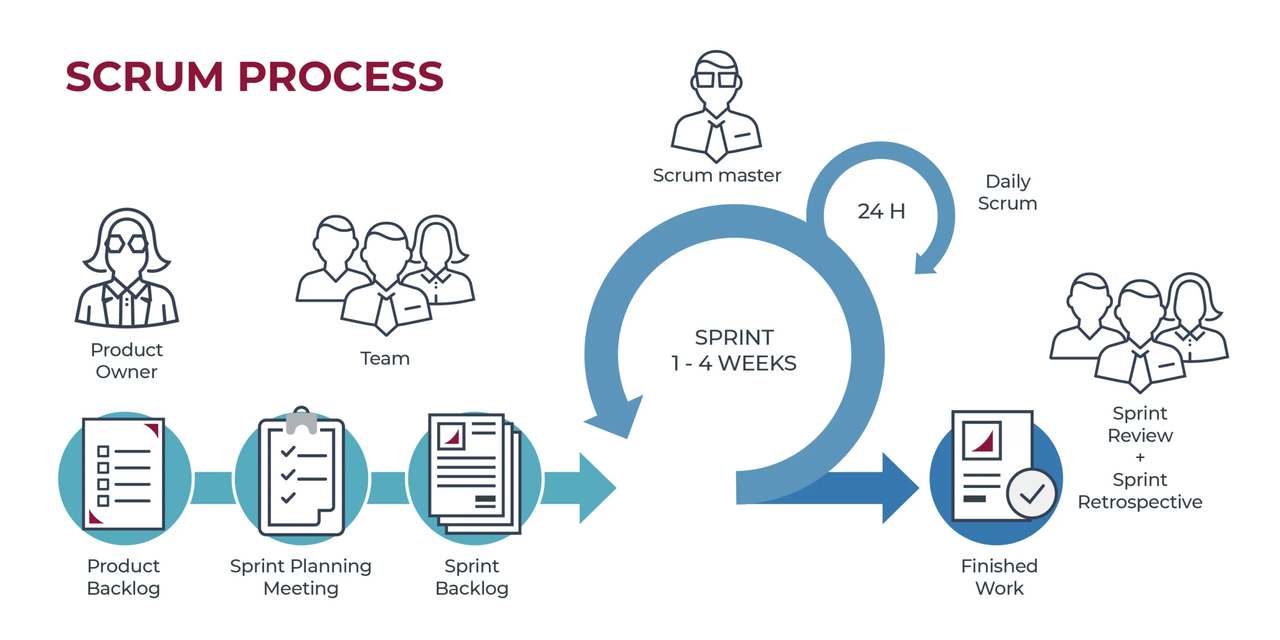
\includegraphics[width=0.75\textwidth]{imagenes/800px-CRISP-DM_Process_Diagram (2).png}
    \caption{Esquema de la Metodologia agil SCRUM}
    \label{fig:scrum}
\end{figure}



Por su parte, CRISP‑DM \ref{fig:crisp} proporciona un proceso de seis fases —\emph{Business Understanding}, \emph{Data Understanding}, \emph{Data Preparation}, \emph{Modeling}, \emph{Evaluation} y \emph{Deployment}— que guía la construcción, validación y puesta en producción de los modelos de clasificación de imágenes. Las entregas de Scrum se alinean con estas fases: los primeros \emph{sprints} se centran en la comprensión del problema clínico y la exploración de los conjuntos de datos; los siguientes abordan la preparación de datos y la experimentación con modelos de segmentación y clasificación; y los últimos se dedican a la evaluación, la integración del modelo en la plataforma y el monitoreo de su desempeño en un entorno real. De esta manera, Scrum aporta el ritmo y la gobernanza del proyecto, mientras que CRISP‑DM asegura la solidez metodológica de las tareas de ciencia de datos, generando una sinergia efectiva entre desarrollo de software y análisis predictivo.


\begin{figure}[H] %si cambia la "H" por "t", se fuerza a que la figura quede arriba de la página
    \centering
    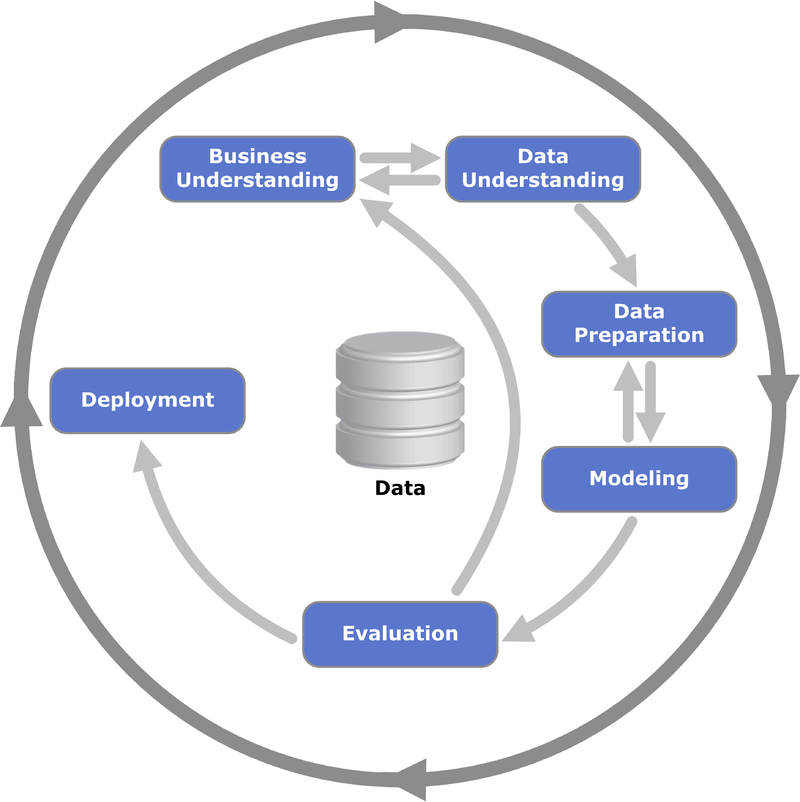
\includegraphics[width=0.41\textwidth]{imagenes/800px-CRISP-DM_Process_Diagram (1).png}
    \caption{Esquema de la Metodologia CRISP-DM}
    \label{fig:crisp}
\end{figure}


